\title{
\huge{\textbf{Surface alignment control of nematodynamics}}\\[1.2cm]
\vspace{0.3in}
\begin{figure}[h]
\begin{center}

\includegraphics[width=0.2\textwidth]{figures/crest}
\end{center}
\end{figure}
\vspace{0.2in}
\large{\href{mailto:c.holmes4@gmail.com}{Christopher John Holmes}}\\
\href{http://emps.exeter.ac.uk/physics-astronomy/}{Department of Physics}\\
\href{http://www.ex.ac.uk}{University of Exeter}\\
\vspace{0.5in}
\Large{Thesis submitted to The University of Exeter \\
for the degree of Doctor of Philosophy} \\[1cm]
\Large{July 2012} }
\author{} \date{}
\maketitle

\newpage
\begin{center}
\thispagestyle{empty}
\vspace*{3cm}
\LARGE{Surface alignment control of nematodynamics}

\vspace*{2cm} {\large Submitted by Christopher John Holmes to the University of Exeter as a thesis for the degree of Doctor of Philosophy in Physics\\ 2012}

\end{center}

\vspace{2cm} {This thesis is available for Library use on the understanding that it is copyright material and that no quotation from the thesis may be published without proper acknowledgement.}

\vspace{1cm} {I certify that all material in this thesis which is not my own work has been identified and that no material has previously been submitted and approved for the award of a degree by this or any other University.}

\begin{flushright}
\vspace{1cm} {Christopher John Holmes\\ 2012}
\end{flushright}

\newpage
%%~~~~~~~~~~~~~~~~~~~~~~~~~~~~~~~~~~~~~~~~~~~~~~~~~~~~~~~~~~~~~~~~~~~~~~~~~~~~~~~~~~~~~~~~~~~~~~~~~~~~~~~~~~~~~~~~~~~~~~~~~~~~~~~~~~~~~~~~~~~~~~~~~~~%
%\newpage \vspace*{8cm}

%%\begin{center} 
%\begin{flushleft}
%I won't even stop\\
%at the valley's brook\\
%for fear that\\
%my shadow\\
%may flow into the world.
%\indent - \textit{\textbf{Eihei D\={o}gen}}
%\end{flushleft}
%\end{center} 
%%~~~~~~~~~~~~~~~~~~~~~~~~~~~~~~~~~~~~~~~~~~~~~~~~~~~~~~~~~~~~~~~~~~~~~~~~~~~~~~~~~~~~~~~~~~~~~~~~~~~~~~~~~~~~~~~~~~~~~~~~~~~~~~~~~~~~~~~~~~~~~~~~~~~%
%\newpage \vspace*{8cm}
%
%\begin{center} 
%\begin{flushleft}
%\textit{`Hearing a cuckoo cry,\\
%I looked up in the direction\\
%Whence the sound came:\\
%What did I see?\\
%Only the pale moon in the dawning of the sky.'}
%\indent - \textit{\textbf{}}
%\end{flushleft}
%\end{center} 

%%~~~~~~~~~~~~~~~~~~~~~~~~~~~~~~~~~~~~~~~~~~~~~~~~~~~~~~~~~~~~~~~~~~~~~~~~~~~~~~~~~~~~~~~~~~~~~~~~~~~~~~~~~~~~~~~~~~~~~~~~~~~~~~~~~~~~~~~~~~~~~~~~~~~%


%%~~~~~~~~~~~~~~~~~~~~~~~~~~~~~~~~~~~~~~~~~~~~~~~~~~~~~~~~~~~~~~~~~~~~~~~~~~~~~~~~~~~~~~~~~~~~~~~~~~~~~~~~~~~~~~~~~~~~~~~~~~~~~~~~~~~~~~~~~~~~~~~~~~~%
%%~~~~~~~~~~~~~~~~~~~~~~~~~~~~~~~~~~~~~~~~~~~~~~~~~~~~~~~~~~~~~~~~~~~~~~~~~~~~~~~~~~~~~~~~~~~~~~~~~~~~~~~~~~~~~~~~~~~~~~~~~~~~~~~~~~~~~~~~~~~~~~~~~~~%
%\newpage \vspace*{8cm}
%
%\begin{center} 
%\begin{flushleft}
%\textit{The moon orbits the earth. High tides and low tides come and go,\\
%the cause being gravity but the reason being nothing.}
%\indent - \textit{\textbf{Alex Garland}}
%\end{flushleft}
%\end{center} 
%
%\newpage
%\vspace*{8cm}
%\begin{center} 
%\begin{flushleft}
%\textit{We keep passing unseen through little moments of other people's lives}\\
%\indent - \textit{\textbf{Robert. T. Persig}}
%\end{flushleft}
%\end{center} 
%
%\newpage \vspace*{5cm}
%\begin{figure}[h]
%\begin{center}
%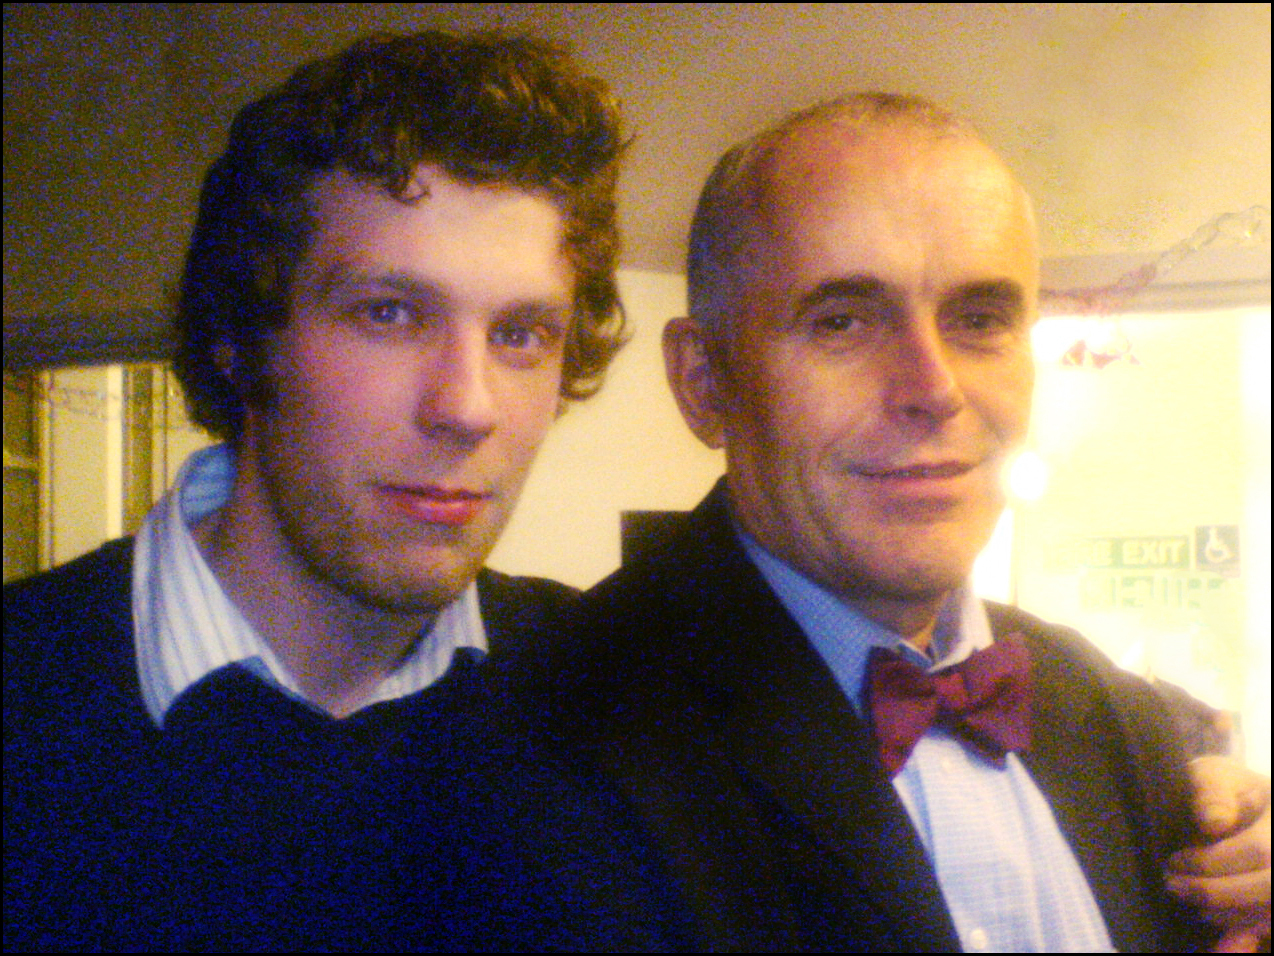
\includegraphics[width=0.5\textwidth]{Figures/alex.jpg}
%\end{center}
%\end{figure}
%\hrule
%\begin{center} 
%Alex, thank you most dearly for your support, mentoring and comic genius throughout my time at Exeter. You were not only my tutor as an undergraduate and my mentor as a postgraduate, you were my friend. I will always smile fondly when I think back on our numerous conversations, which almost always ended in a discussion about the pants I was wearing.\\
%\vspace*{0.5cm}
%Alex, you are sorely missed.\\
%\vspace*{0.5cm}
%\indent\textbf{Alex Savchenko ( - 27.6.2010)}
%\end{center} 
%\chapter*{Abstract}
%{Since their discoevry in...}
%
%%~~~~~~~~~~~~~~~~~~~~~~~~~~~~~~~~~~~~~~~~~~~~~~~~~~~~~~~~~~~~~~~~~~~~~~~~~~~~~~~~~~~~~~~~~~~~~~~~~~~~~~~~~~~~~~~~~~~~~~~~~~~~~~~~~~~~~~~~~~~~~~~~~~~%
\chapter*{Abstract}
The primary study of this thesis is the response of the nematic director to pressure driven flow. Dynamic flow experiments using optical conoscopy and pressure gradient measurements are used to explore the physics behind the flow alignment seen to occur for some nematic liquid crystals. New research into the techniques and methods for aligning the director at a glass interface is also presented, the results of which are used towards the latter end of this thesis in the production of a highly novel flow cell. A bespoke technique for fabricating robust liquid crystal flow cells is also presented.

The observation of flow alignment for the nematic liquid crystal 5CB is detailed for pressure driven flow via optical conoscopy when the director is initially aligned planar homogeneously at $45^{\circ}$ to the direction of flow. The results of this experiment are compared to the theory of Ericksen and Leslie through a one dimensional dynamic model that provides simulated director profiles and corresponding simulated conoscopic images. Good agreement between the data and simulation is observed, whereby the director is seen to rotate to become parallel to the flow direction whilst exhibiting no net tilt distortion at all flow rates.

The presence of small surface pretilt from a rubbed planar aligning polyimide layer and its effect on director rotation is also examined for cells that are rubbed in both the parallel and anti-parallel directions. The result observed is a striking difference in the mean director rotation when initially aligned close to normal to the direction of flow. The results of these experiments are also compared to the theory of Ericksen and Leslie through the one dimensional dynamic model. Good agreement is seen, highlighting the dramatic effect that a small amount of surface pretilt can have on the overall director orientation, whilst also demonstrating the need for caution when assuming that rubbed conventional alignment techniques provide true planar orientation.

Two methods for producing intermediate or large pretilt angles at liquid crystal alignment surfaces are also examined. Here, two recipes involving the commercial polyimides Nissan SE-1211, Nissan SE-130 and Nissan SE-4811 are experimentally investigated, with results showing the ability to tune the director pretilt angle as a function of the rubbing strength used to align the sample. The results also show an interesting dependance on the material upon which the aligning layer is deposited for the recipe involving Nissan SE-1211. Here, vastly different pretilt angles are observed for cells constructed with glass and indium tin oxide (ITO) layers.

Finally, the large pretilt angles produced from the recipes mentioned above are also used to fabricate pressure driven flow cells exhibiting large pretilt angles on both surfaces, constraining the director to align in a splayed state. When aligned parallel to the flow direction, experiments examining the valve-like nature of the director profile suggest that a preferential flow direction exists in what here is termed the `diode cell'. Measurements of the pressure gradient required to achieve a constant volumetric flow rate through the cell are compared for flow in both directions relative to the splayed director profile. A striking difference is observed for flow `with' the splay and `against' the splay, leading to the realisation of a cell exhibiting a preferential flow direction through surface treatment. Again, results are compared to the theory of Ericksen and Leslie through the one dimensional dynamic model, showing good agreement.



\newpage
\tableofcontents*
\listoffigures
\listoftables

\chapter*{Acknowledgements}
I would like to take this opportunity to say a genuine and heart-felt thank you to the many people who helped me on the way to finally completing this thesis.

Firstly, of course, I thank my supervisor Professor Roy Sambles. The road to this thesis hasn't always been easy, but Roy has helped me put things into perspective on more than one occasion, and for that I am truly grateful. It has not only been your ability to instantly spot the solution to my problems, but also your ability to instantly spot when I've been surfing rather than in the lab, that has kept me on my toes throughout the last three years. Thank you.

Secondly, I must say a special thank you to Stephen Cornford. If it were not for both your immense understanding of liquid crystal dynamics and your immense ability to explain complex problems to me in a way in which I can understand, this Ph. D would not have been possible. Your razor sharp wit has also not gone un-noticed. I must also apologise for the barrage of messages you received once I'd started writing up this thesis, when I was having a panic attack almost daily. Thank you Steph.

I must also say a special thank you to the displays team at Hewlett Packard Labs in Bristol. I gratefully acknowledge the genuine interest and help that I received at our CASE meetings. I can honestly say that I felt welcome and part of the team almost instantly. A special mention must go to Tim Taphouse for being an all round source of technical expertise as well as being a fantastic mentor, and also to Steve Kitson for always taking the time to help out and always providing the solution to the problem at hand. Fantastic input was almost always provided by everyone in the group with particular reference to Adrian Geisow and Chris Newton. Of course, the ECLC 2011 in Slovenia would not have been as enjoyable without the `mothering' provided by Suzanna Klein and the perpetual moaning provided by Rob `hang-time' Greasty. Thank you.

 A big thank you must also go to Benny Hallam for being very understanding in giving me time to finish writing when I started work in Cornwall.

Next, as is customary, I would like to thank the more senior members of the Electromagnetic Materials Group at Exeter. Firstly, what can I say? Matthew (Lockers, Lockertron, Stocker, LockHeart) Lockyear RCE. Perhaps the less said here the better. Just remember this, `\textit{what's said in the water, stays in the water}'. Next I must say thank you to Alistair `Hello there' Hibbins for all the comic moments and home-brew help. I can't wait to see what you cook up for the next Great Physics Beer Festival. Thank you to Ian `Hoop-dream' Hooper NRC. For you I have just one question, just one, it's a question that everyone is dyeing to know the answer too, something that I haven't been brave enough to ask you over the last three years ................... vodka ball? A special thank you also to both Fuzi and Lizhen, whether we were discussing my previous girlfriends, or a bowl of 2000 year old soup from an ancient chinese grave, I was always having fun. Sharon Jewell for all the help and advice at the start of my `three years', it's fair to say that you taught me almost everything I know about making liquid crystal cells, and you were right, about 1 in 4 did work! Tim Atherton for your `long range' helpful conversations, listening ear and computational expertise! Euan Hendry for regularly taking all my money in late night poker sessions. Pete V for the sound life advice and that one good surf at Putsborough, hopefully we'll get in again sometime. Bill Barnes for not only being an all round source of help, but for being my first tutor as an undergraduate physicist and firmly setting me on the path to continuing in Physics. Andy Murray for tea time chat and that one good surf at Dawlish Warren, keep it up (the sea will get warmer in the summer)! Tomeck for all the figure conversion that you made possible. Much appreciated! Evgenny Sirotkin for being a fantastic Russian role model. I've never known anyone with a stronger hand shake or a firmer hug and pat on the back. Tom Isaac for being a source of much humour and good will, and to Nick Cole, without you I wouldn't have any samples or any shiny metal things to play with. We started at near enough the same day, and I have to say it's gone very fast, but thank you for all the technical expertise and advice. I must also say a big thank you to Alan Usher for agreeing to be my mentor at such short notice, and after just one meeting, helping me feel much better about my Ph. D.

Throughout my undergraduate time at Exeter, I made some great friends in Physics that also went on to complete their Ph. Ds here at Exeter. These are Lemmy Steve, Chris `Buzza' Burrows and James Edmunds. So I must say a big thank you to you guys for helping me through my time here as a Ph. D student. In particular Lemmy Steve for all the good years as MPhys lab partners and hopefully many more good years to come!

Next I come to a special section of my acknowledgements. Team Basement. When I first started my Ph. D, a select few were chosen to dwell in the basement of the Physics department. Without natural light, cleanliness, or a chance of escape, we forged a special bond that many basement dwellers before us have also shared. So I must say a massive thank you to the original Team Basement for helping to keep me sane and providing me with some of the best memories of my time at Exeter. James Parsons, Caroline `\textit{Simon, side step to your left}' Pouya (aka Jupiter) and Edmund Stone. Ed, I must say a special thank you for not actually killing me, and for all the help with R during the early days. You were a fantastic human drum kit and I hope our friendship continues long after our time at Exeter! Caroline I must also say thank you for expanding my musical horizons and making me a better all round individual. Maybe someday you'll like Radiohead?

Along with Team Basement, there were many new Ph. D starters in 2008. Over the last three years I feel I've made good friendships with all of you and would like to say a big thank you to Matt `Biggatronic' Bigginton, you adonis! Mel Taylor, for helping me calm down when I started to panic about this thesis. Celia Butler for being an all round source of information and help, I'd love to go gliding some day. Last but not least, a special mention must go to Helen Rance RC for eating all my chocolate bourbons and teaching me how to cook, a bit. 

Also, during my three years as a post graduate student, I have met many new starters. Unfortunately we haven't been able to spend a long time together, but I would like to say thank you to Dmitry Polyushkin, Lizzy Brock, Simon Berry, Chinna Devarapu (you have the best laugh in the world!), Al Murray, Matt Nixon, Tim Starkey RC and Joe Blackman, who made me realise that not everything is lost! 

Who am I missing? I'm sure I'm missing someone important...oh yes! That's right, Alfred John Lethbridge. Well, what can I say? It seems strange to acknowledge you, since we are in fact the same person, but, `\textit{sometimes....not always....but sometimes}'. Seriously, thanks for the sound advice and brilliant memories over the last two years. See you in China.

Penultimately I would like to thank The Stormers with which I had the insurmountable pleasure of living (and working) with for 2 years. Namely, Dr. Ciaran `Stewstorm' Stewart RC, Thomas `Constorm' Constant RC and Peter `Halestorm' Hale. Ciaran, you are a fantastic chef and a fantastic person. Thank you for all the bacon sandwiches and cups of tea. Not only that, but for all the surfing memories and BBQs at Radstations. I will, forever, remember the day of ball-ache. Tom, you are in some ways, the epitamy of what a Stormer should be. A gentleman and a scholar. Thanks for the t-shirt which i'll never wear again, and maybe someday you'll be the subject of an award winning National Geographic photo. Finally Pete, i'm writing this with my chordorouy trousers on. Perhaps we should make the angle again? Definitely DON'T come in (thanks for the tea).

Finally I'd like to say a huge thank you to my Mum, Dad and Brother. If it wasn't for the science open day at Ridgeway school all those years ago, I may never have experienced the joy of watching a ping pong ball being levitated by a jet of air from a vacuum cleaner in reverse. That means I may have never developed an interest in Physics! But seriously, thank you for the constant love, support, help and advice.


%\newpage
%%~~~~~~~~~~~~~~~~~~~~~~~~~~~~~~~~~~~~~~~~~~~~~~~~~~~~~~~~~~~~~~~~~~~~~~~~~~~~~~~~~~~~~~~~~~~~~~~~~~~~~~~~~~~~~~~~~~~~~~~~~~~~~~~~~~~~~~~~~~~~~~~~~~~%
\newpage \vspace*{8cm}
\begin{center} 
\begin{flushleft}
\textit{The pessimist complains about the wind;\\
the optimist expects it to change;\\
the realist adjusts the sails\footnote{Never has a single quote made more sense to me than now, writing from the vantage point of a completed Ph.D thesis}\\}
\indent - \textit{\textbf{William Arthur Ward}}
\end{flushleft}
\end{center} 



%\newpage \vspace*{8cm}
%\begin{center} 
%\begin{flushleft}
%\textit{As a child I had dreams of levitation.\\In these dreams I could float off the ground only when no one watched.\\The ability would leave me just when someone looked.\\}
%\indent - \textit{\textbf{Robert C. Mason}}
%\end{flushleft}
%\end{center} 
%\newpage

%\newpage \vspace*{8cm}
%\begin{center} 
%\begin{flushleft}
%\textit{Today we cannot see whether Schr\"{o}edinger's equation contains frogs, musical composers, or morality - or whether it does not. We cannot say whether something beyond it like God is needed, or not. And so we can all hold strong opinions either way.}
%\indent - \textit{\textbf{Richard Feynman}}
%\end{flushleft}
%\end{center} 
%\newpage